\documentclass[tikz, border=0pt]{standalone}
\usepackage{tikz}
\usetikzlibrary{arrows,automata,positioning}

\begin{document}
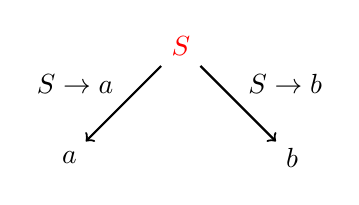
\begin{tikzpicture}[node distance=2cm, thick, auto]
% draw the states
\node[red] (S) {\(S\)};
\node (a) [below left of=S] {\(a\)};
\node (b) [below right of=S] {\(b\)};
% draw the edges
\path[->] 
(S) edge node [swap] {\(S \to a\)} (a)
(S) edge node {\(S \to b\)} (b)
;
\end{tikzpicture}
\end{document}